\documentclass[border=2pt]{standalone}
\usepackage{amsmath}
\usepackage{tikz}
\usetikzlibrary{calc,shapes.misc}
\begin{document}
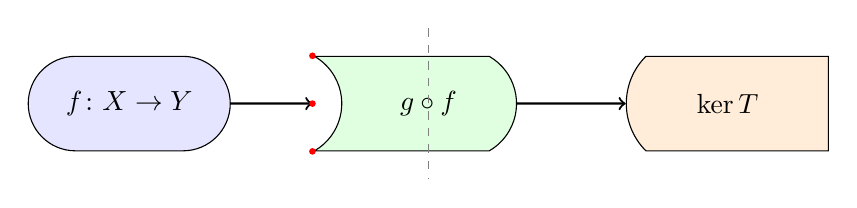
\begin{tikzpicture}[every node/.style={draw,rounded rectangle,minimum width=28mm,minimum height=12mm}]
  \node[fill=blue!10,rounded rectangle arc length=180] (a) at (0,0) {$f\colon X\to Y$};
  \node[fill=green!12,rounded rectangle arc length=120,
    rounded rectangle west arc=concave] (b) at (3.8,0) {$g\circ f$};
  \node[fill=orange!15,rounded rectangle arc length=90,
    rounded rectangle east arc=none] (c) at (7.6,0) {$\ker T$};
  \draw[->,thick] (a) -- (b);
  \draw[->,thick] (b) -- (c);
  \fill[red] (b.north west) circle (1.2pt);
  \fill[red] (b.west) circle (1.2pt);
  \fill[red] (b.south west) circle (1.2pt);
  \draw[dashed,gray] ($(b.north)+(0,.35)$) -- ($(b.south)+(0,-.35)$);
\end{tikzpicture}
\end{document}
